\documentclass[12pt]{ruthesis}

\usepackage{amsmath}
\usepackage{amssymb}
\usepackage{mathtools}
\usepackage{physics}
\usepackage{multirow}
\usepackage{float}
\usepackage{graphicx}
%\usepackage{braket}
\usepackage{hyperref}
\usepackage{color}
\usepackage{bm}
\usepackage[]{siunitx}
\usepackage[]{cleveref}
\usepackage[style=phys,
			articletitle=false,
			biblabel=brackets,
			chaptertitle=false,
			pageranges=false]{biblatex}

% Footnotes are continuously labeled (e.g. without regard for sections, chapters, etc.). 
\usepackage{chngcntr}
\counterwithout{footnote}{chapter}
\interfootnotelinepenalty=10000 %Supposed to keep footnotes from being split

% Additional options
\DeclareSIUnit\atoms{atoms}
\addbibresource{bibliography.bib}

% cleveref options
\crefname{equation}{Eq.}{Equations}
%\crefname{pluralequation}{Eqs.}{Equations}


% Macros
\newcommand{\tsup}{\textsuperscript}													% superscript outside math mode.
\newcommand{\tsub}{\textsubscript}														% subscript outside math mode.
\newcommand{\Sr}[1]{\tsup{#1}\textnormal{Sr}}											% {}^{xx}Sr outside math mode.
\newcommand{\Srion}[1]{\textnormal{Sr}\tsup{#1}}										% {}Sr^{xx} outside math mode.
\newcommand{\Li}[1]{\tsup{#1}\textnormal{Li}}											% {}^{xx}Li outside math mode.
\newcommand{\SLJ}[3]{\tsup{#1}\textnormal{#2}\tsub{#3}}
\newcommand{\SLJF}[4]{\tsup{#1}\textnormal{#2}\tsub{#3}\textnormal{, }{F = {#4}}}
\newcommand{\nSLJ}[4]{{#1}\textnormal{ }\SLJ{#2}{#3}{#4}}
\newcommand{\nSLJm}[5]{{#1}\textnormal{ }\SLJ{#2}{#3}{#4}\textnormal{, }{m_J = {#5}}}
\newcommand{\nSLJF}[5]{{#1}\textnormal{ }\SLJ{#2}{#3}{#4}\textnormal{, }{F = {#5}}}

\newcommand{\iu}{{i\mkern1mu}}

\title{PhD Thesis Title Here}
\author{Roger Ding}
\department{Applied Physics}
\school{William Marsh Rice University}
\degree{Doctor of Philosophy}

\committee{
	F. Barry Dunning, Advisor \\
	Sam and Helen Worden Professor of Physics
	\and
	Thomas C. Killian, Co-advisor \\
	Professor of Physics and Astronomy
	\and
	Junichiro Kono \\
	Professor of Electrical and Computer Engineering \\
	Professor of Physics and Astronomy
}

\address{Houston, Texas}
\donemonth{April}
\doneyear{2008}
\makeindex

\begin{document}

%%%%%%%%%%%%%%%%%%%%%%%%%%%%%%%%%%%%%%%%%%%%%%%%%%
% Front-matter

\begin{frontmatter}
	\pagenumbering{roman}
	%\makecover
	\maketitle
	This dissertation describes the development of an apparatus to undertake spectroscopic studies of \Sr{87} Rydberg states and their application in the production of ultra-long-range Rydberg molecules (ULRRMs). 
Most previous spectroscopic studies of strontium have been performed with the bosonic isotope \Sr{88} which has no nuclear spin ($I = 0$), resulting in a relatively simple and well-understood Rydberg excitation spectrum. 
In contrast, fermionic \Sr{87} has a large nuclear spin ($I = {9}/{2}$) that leads to strong hyperfine interactions which greatly complicate the Rydberg excitation spectrum.
In order to understand the Rydberg states in \Sr{87}, two-photon spectroscopy was performed to measure and identify the $\nSLJ{5sns}{3}{S}{}$ and $\nSLJ{5snd}{3}{D}{}$ hyperfine Rydberg states for $30 \lesssim n \lesssim 99$.
Working with theory collaborators, a detailed understanding of how the hyperfine interaction affects the Rydberg levels is developed and used to extract revised quantum defects.

The detailed understanding of the \Sr{87} hyperfine Rydberg structure was then utilized to produce the first ULRRMs in a fermionic gas.
Unlike traditional molecular binding mechanisms, ULRRMs comprise of one or more ground-state atoms embedded in the electron cloud of a Rydberg atom with the entire system bound together through the weak Rydberg electron-neutral atom scattering. 
Therefore, production of ULRRMs is dependent on both the principal quantum number ($n$) of the parent Rydberg atom and the initial spatial distribution of atoms. 
At low temperatures, the effects of quantum statistics becomes important and result in bunching (bosons) and antibunching (fermions).
These differences in spatial distributions can influence the excitation rates of ULRRMs. 
Current progress in exploring the role of quantum statistics in the excitation of ULRRMs using cold, dense strontium gases is described, with an emphasis on \Sr{87}, and how such measurements can be used to extract the pair correlation function $g^{\pqty*{2}}\pqty*{R}$.
	\begin{acknowledge}

Acknowledgments go here. 

\end{acknowledge}
	\tableofcontents
	\listoffigures
	\listoftables
\end{frontmatter}


\pagenumbering{arabic}

\linespacing{1.7}

%%%%%%%%%%%%%%%%%%%%%%%%%%%%%%%%%%%%%%%%%%%%%%%%%%
% Chapters

\chapter{Introduction}

***************************************************

*********** NOTES TO SELF, REMOVE LATER ***********

(0) Long-range and anisotropic interactions

(0a) Few-/Many-body physics

(0b) Ultra-long-range Rydberg molecules

(1) Spectroscopy

(2) Effects of quantum statistics -- use Joe's figure?

Add in repumper spectrum.

***************************************************

***************************************************



The ability to produce ultracold samples paved the way towards achievement of quantum degenerate gases of atoms which are ideal systems for studying quantum interactions. 
From the observation of BEC-BCS crossover \cite{Chen2005.PR.412.1, Gurarie2007.JAOP.322.2, Bourdel2004.PRL.93.050401}, superfluid to Mott insulator transition in an optical lattice \cite{Greiner2002.Nature.415.39}, and the formation of matter-wave solitons \cite{Strecker2002.Nature.417.150, Khaykovich2002.Science.296.1290}, most of the work in these systems have been based on a short-range, isotropic contact interactions described by the pseudopotential \cite{Pethick.BEC}
\begin{equation}
	U\pqty{\va{r}}	=	\frac{4 \pi \hbar^2}{m} a_{s} \delta\pqty{\va{r}}
\end{equation}
where $a_{s}$ is the $s$-wave scattering length.
This effective interaction requires the atomic wave functions to overlap. 

An important recent trend in the field of ultracold atomic gases is the study of systems with long-range interactions which can typically be expanded as \cite{Pethick.BEC}
\begin{equation}
	U\pqty{\va{r}}	=	\sum^{\infty}_{k=1} \frac{C_{k} \pqty{\va{r}}}{r^{k}}
\end{equation}
with the ``long-range'' coming from the $U \sim {1}/{r^{k}}$ dependence. 
Depending on the type of interaction (e.g., Coulomb $k = 1$, dipole-dipole $k = 3$, van der Waals $k = 6$), the potentials can be isotropic or anisotropic, providing additional richness to quantum systems and the opportunity to study a wide variety of phenomena including applications towards quantum computing \cite{Jaksch2000.PRL.85.2208, DeMille2002.88.067901}, quantum simulation \cite{deLeseleuc2018.PRL.120.113602, Schauss2018.QST.3.023001}, and tests of theories **** SOURCES? ****
There are several methods for incorporating long-range interactions in to ultracold systems with some of the most prominent being \cite{Lahaye2009.RPP.72.126401}: 
\begin{description}
	\item[Polar molecules]
		These molecules can have large (permanent) electric dipole moments \cite{Aymar2005.JCP.122.204302} and can, ignoring chemical reactions, have extremely long lifetimes. 
		The drawback is that the additional complexity typically makes it very difficult to produce ultracold and quantum degenerate samples. 
		In spite of these challenges, a degenerate Fermi gas of {{\tsup{40}\text{K}}{\tsup{87}\text{Rb}}} was recently achieved by associating atoms from a BEC of {\tsup{87}\text{Rb}} and a degenerate Fermi gas of {\tsup{40}\text{K}} \cite{DeMarco2019.Science.363.853}. 
		Steady progress continues to be made in the direct laser cooling of molecules as well \cite{Anderegg2018.NatPhys.14.890}.
	\item[Magnetic atoms]
		Atoms themselves can have permanent dipole moments which can be exploited to study long-range interactions. 
		Quantum degeneracy has been reached with chromium \cite{Griesmaier2005.PRL.94.160401, Naylor2015.PRA.91.011603}, erbium \cite{Aikawa2012.PRL.108.210401, Aikawa2014.PRL.112.010404}, and dysprosium \cite{Lu2011.PRL.107.190401, Lu2012.PRL.108.215301}.
		Although simpler than molecules, their dipolar interactions are limited by the magnetic moment of atoms and typically requires tuning the short-range interaction strength to be weaker than the dipole-dipole interaction to observe their effects.
		There's also been a recent proposal for creating ultracold dysprosium atoms which exhibit an electric dipole moment in addition to the magnetic dipole moment \cite{Lepers2018.PRL.121.063201}.
	\item[Coupling atoms to a high-finesse cavity]
		An ingenious way of inducing long-range interactions in atomic systems is by placing the atoms in a high-finesse optical cavity such that they couple to the cavity mode which in turn causes the atoms to experience position-based forces \cite{Baumann2010.Nature.464.1301, Mottl2012.Science.336.1570}.
		Although the interactions are (essentially) infinite-range, they are likely to be restricted to only that case. 
		They are also constrained by the geometry of the experiment which could make it difficult to tune between isotropic and anisotropic interactions.
	\item[Rydberg states]
		Highly excited Rydberg states of atoms (and molecules) with principal quantum number $n \gg 1$ can also exhibit strong dipole interactions \cite{Gallagher1994.RydbergAtoms} and have even been observed in solid state systems \cite{Kazimierczuk2014.Nature.514.343}. 
		Since many of the properties of Rydberg atoms scale with $n$, the Rydberg-Rydberg interactions can be tuned in strength and anisotropy by simply exciting different Rydberg states. 
		Rydberg atoms can also leverage well-established techniques for producing quantum degenerate gases of atoms so that their interactions can be readily incorporated to existing setups. 
		The major disadvantage of Rydberg systems are their sensitivities to stray electric fields and the limited Rydberg lifetimes due to both blackbody and Rydberg-Rydberg interactions. 
\end{description}
This thesis will be focused on the latter by studying Rydberg systems in ultracold strontium gases. 
Most ultracold Rydberg experiments have predominantly focused on exciting alkali metal atoms (primarily rubidium and cesium with a growing interest in potassium).
With their hydrogen-like electronic structure, there are well-established methods for both calculating their properties (e.g., see \cite{Sibalic2017.CPC.220.319}) and techniques for producing ultracold and quantum degenerate gases.
But since the interactions are long-ranged, generally comparable to the inter-particle separation in the gas, the particular atomic species used should only affect the details of the interactions but not the overall form. 
As will be discussed below, strontium has some properties which make it a very advantageous system for studying Rydberg physics. 

\section{Rydberg Atoms}

A Rydberg atom can be loosely defined as an atom in an excited state with very large principal quantum number ($n$), i.e., $n \gg 1$. 
Starting in the late {1800's}, it was observed that the wavenumbers of atomic spectra could be described by the formula
\begin{equation}
	\label{eq:Rydberg_formula}
	\nu_{l} = \nu_{\infty,l} - \frac{R}{\pqty{n-\delta_{n,l}}^2}
\end{equation}
where $\nu_{\infty,l}$ is the series limit, $\delta_{n,l}$ is a ``quantum defect'', and $R$ is the Rydberg constant \cite{Rydberg1890.Recherches, Rydberg1890.PM.29.331, Gallagher1994.RydbergAtoms}. 
This is the Rydberg formula.
Conceptually, a Rydberg atom can be thought of as being comprised of a core ion and a highly-excited valence electron which spends the majority of its time far away from the core.
As a result, the Rydberg electron rarely interacts with the core which allows its effects to be characterized by (nearly) constant parameter $\delta_{n,l}$.
While the details of the core ion and electrons are important, which causes $\delta_{n,l}$ to vary from atom-to-atom and from orbital-to-orbital, it generally does not have a large effect on the overall properties of the Rydberg atom.

Although the details of the core are usually small, the principal quantum number does greatly affects the atomic wave function. 
As a result, it sets the energy scale for many interactions which leads to the properties of Rydberg atoms become exaggerated when $n$ becomes large.
\Cref{tab:Rydberg_n-scaling} gives the $n$ dependence for a few Rydberg atoms properties. 
\begin{table}[h]
	\centering
	\caption[]{
		\label{tab:Rydberg_n-scaling}
		Some properties of Rydberg atoms \cite{Gallagher1988.RPP.51.143, Gallagher1994.RydbergAtoms, Camargo2016.PRA.93.022702, Ding2018.PRA.98.042505}.
		*** Double check values!! ***}
	\begin{tabular}{@{}cccc@{}}
		\toprule
		Property					& $n$ scaling	& {Na} : {$\nSLJ{10d}{2}{D}{}$}					& {Sr} : {$\nSLJ{5s38s}{3}{S}{1}$}	\\
		\midrule
		Binding energy				& $n^{-2}$		& $\SI{0.14}{\eV}$								& $\SI{0.01134}{\eV}$				\\
		Coulomb splitting			& $n^{-3}$		& $\SI{0.023}{\eV}$								& $\SI{0.00058}{\eV}$				\\
		Fine structure splitting	& $n^{-3}$		& $\SI{-92}{\MHz}$								& $\SI{2.56659}{\GHz}$				\\
		Orbital radius				& $n^{2}$		& $\SI{147}{\bohr}$								& $\SI{1799}{\bohr}$				\\
		Radiative lifetime			& $n^{3}$		& $\SI{1}{\us}$									& $\SI{21}{\us}$					\\
		Polarizability				& $n^{7}$		& $\SI{0.21}{\MHz\per(\volt\per\cm)\squared}$	& 									\\
		Ionization field			& $n^{??}$		&												& 									\\
		\bottomrule
	\end{tabular}
\end{table}

\subsection{Ultralong-Range Rydberg Molecules (ULRRMs)}

One key aspect to focus on from \cref{tab:Rydberg_n-scaling} is that size of a Rydberg atom increases very quickly with $n$. 
In a dense enough gas, $\ev*{r} \sim n^{2}$ can quickly become comparable to (or larger than) the interparticle separations.
It was in this context, when an atom (or multiple atoms) could be located inside the Rydberg electron's orbit, that a density-dependent shift was first observed in the spectral lines of alkali atoms with the direction of the shift, relative to the unperturbed atomic line, also depended on the buffer gas used \cite{Amaldi1934.NC.11.145, Amaldi1934.Nature.133.141, Liebisch2016.JPB.49.182001, Shaffer2018.NatComm.9.1965}.
\begin{figure}[htbp]
	\centering
	\includegraphics[keepaspectratio, width=\textwidth, height=\textheight]{introduction/rydberg_molecules/orbital_radius-density_n-scaling.pdf}
	\caption[]{
		\label{fig:orbital_radius-density_n-scaling}
		Orbital radius $\ev{r}$ and the corresponding density ${1}/{\ev{r}^3}$ for a strontium Rydberg atom in the $\nSLJ{5sns}{3}{S}{1}$ state.
		The shaded region represents the range of densities typically achievable in ultracold strontium experiments with a maximum of about $\SI{1E15}{\per\cm\cubed}$ occurring in a \Sr{88} BEC \cite{Yan2013.PRL.110.123201, Stellmer2014.arXiv.1307.0601}.}
\end{figure}
\Cref{fig:orbital_radius-density_n-scaling} shows $\ev{r}$ and ${1}/{\ev{r}^3}$ for a strontium atom in the $\nSLJ{5sns}{3}{S}{1}$ state and the typical densities achievable in ultracold gas experiments.
Notice that, even for modest principal quantum numbers and densities, it's easily possible to excite Rydberg atoms much larger than the interparticle separations.

This shift was first explained by Fermi \cite{Fermi1934.NC.11.157}, and later generalized by Omont \cite{Omont1977.JPF.38.1343}, to be the result of low-energy scattering of the Rydberg electron off nearby neutral atoms, formulating the electron-atom interaction with the pseudopotential \cite{DeSalvo2015.PRA.92.031403, Liebisch2016.JPB.49.182001, Shaffer2018.NatComm.9.1965}
\begin{equation}
	V\pqty*{\va{R}}
		=	\sum_{i} \frac{2 \pi \hbar^{2} A_{s}\bqty*{k\pqty*{\va{R}}}}{m_{e}} \delta\pqty*{\va{r}_i - \va{R}}
			+ \frac{6 \pi \hbar^{2} A_{p}^{3}\bqty*{k\pqty*{\va{R}}}}{m_{e}} \overleftarrow{\grad}{\delta\pqty*{\va{r}_i - \va{R}}}\overrightarrow{\grad}
\end{equation}
where $\va{r}_{i}$ is the position of the Rydberg valence electron(s) and $\va{R}$ is the position of the ground-state atom from the Rydberg core. 
On the right hand side, the first term is the $s$-wave contribution and the second term is the $p$-wave contribution with momentum-dependent scattering lengths $A_{s}\pqty{k}$ and $A_{p}\pqty{k}$, respectively, and the semiclassical Rydberg electron momentum given by $\hbar {k \pqty{\va{r}}} = \sqrt{2 m_{e} \bqty{{e^2}/{\pqty{4 \pi \epsilon_0 \va{r}}} - E_{b}}}$ for the unperturbed Rydberg electron binding energy $E_{b}$ \cite{DeSalvo2015.PRA.92.031403}.
Evaluating the interaction with the Rydberg electron wave function $\Psi_{ns}$ leads to \cite{DeSalvo2015.PRA.92.031403}
\begin{equation}
	V\pqty*{\va{R}}
		\simeq	\sum_{i} \frac{2 \pi \hbar^{2} A_{s}\pqty*{k}}{m_{e}} {\abs*{\Psi_{ns}\pqty*{\va{r}_{i} = \va{R}}}^2}
				+ \frac{6 \pi \hbar^{2} A_{p}^{2}\pqty*{k}}{m_{e}} {\abs*{\grad \Psi_{ns}\pqty*{\va{r}_{i} = \va{R}}}^2}
\end{equation}
**** NEED TO DOUBLE CHECK THE ABOVE EQUATIONS ****
A very nice derivation of the interaction is presented in \cite{Bendkowsky2010.PhD}\footnote{She references \cite{Balewski2009.Diploma} which has more details of Fermi's approach.}.

We are particularly interested in the case when, in the low-energy scattering regime, $A_{s} < 0$ because the interaction is attractive and can lead to the formation of bound states nearby ground state atoms in the Rydberg electron wave function.
These are known as ``ultralong-range Rydberg molecules''\footnote{Other objects can also be called ``Rydberg molecules'' (e.g., a molecule electronically excited to a high principal quantum number) but for the purposes of this thesis, a Rydberg molecule refers to the binding of neutral atoms to a Rydberg atom due to scattering.} (ULLRMs) with the binding mechanism, instead of being ionic or covalent, is due to Rydberg-electron neutral scattering and were theoretically predicted by Greene et al., in {2000} \cite{Greene2000.PRL.85.2458}. 
The first experimental detection of ULLRMs occurred in \Rb{87} \cite{Bendkowsky2009.Nature.458.1005} with subsequent observations in {Cs} \cite{Tallant2012.PRL.109.173202} and {Sr} \cite{DeSalvo2015.PRA.92.031403}. 

\Cref{fig:n34_rydberg_molecule_wave_functions_and_spectra} provides an example of the molecular potential and the resulting radial vibration wave functions along with the spectroscopic signal. 
\begin{figure}[htbp]
	\centering
	\includegraphics[keepaspectratio, width=\textwidth, height=\textheight]{introduction/rydberg_molecules/n34-wave_functions_and_spectra/n34-wave_functions_and_spectra.pdf}
	\caption[]{
		\label{fig:n34_rydberg_molecule_wave_functions_and_spectra}
		(Top) Calculated molecular potential ($V$) for a $\nSLJ{5s34s}{3}{S}{1} + \nSLJ{5s^2}{1}{S}{0}$ atom pair together with the radial vibrational wave functions for the $\nu = 0$ to $\nu = 4$ vibrational states.
		(Bottom) Rydberg molecule spectra in unpolarized gas of \Sr{87} and highlighting various dimer vibrational states.}
\end{figure}


****** 

MENTION INTERACION ENERGIES AND NEEDING ULTRACOLD SAMPLES

***********

OFR with Rydberg molecules \cite{Thomas2018.NatComm.9.2238}.

\section{Strontium Rydberg Atoms}

Strontium offer several benefits over the alkali atoms with perhaps the most obvious, as seen in \cref{fig:sr_levels-boson}, being the singlet and triplet Rydberg series due to the two valence electrons.
\begin{figure}[h]
	\centering
	\includesvg[keepaspectratio, width=\textwidth, height=\textheight]{introduction/sr_levels/sr_levels-boson.svg}
	\caption{
		\label{fig:sr_levels-boson}
		Grotrian diagram for (bosonic) strontium (\Sr{88} in particular).
		*** FIX FIGURE -- CHECK SOUMYA'S UPDATED CODE ***.}
\end{figure}
Starting from the $\nSLJ{5s^2}{1}{S}{0}$ ground state, a two-photon excitation can be used to access the myriad of $\SLJ{1}{S}{0}$, $\SLJ{3}{S}{1}$, $\SLJ{1}{D}{2}$, and $\SLJ{3}{D}{1,2,3}$ Rydberg levels.
In addition to the anisotropies of a particular Rydberg orbital, the $C_{6}$ coefficients have been calculated for these states and exhibit both attractive ($C_{6} < 0$) and repulsive ($C_{6} > 0$) interactions \cite{Vaillant2012.JPB.45.135004}. 
The second electron does introduce additional complexity (``richness'') as well due to there being multiple Rydberg series which can interact and typically requires multichannel quantum defect theory (MQDT) \cite{Gallagher1994.RydbergAtoms, Vaillant2014.JPB.47.155001, Robicheaux2018.PRA.97.022508} and/or two-active electron (TAE) models \cite{Ye2013.PRA.88.043430} to described the spectra.
There is also the opportunity to produce doubly-excited and autoionizing states \cite{Gallagher1994.RydbergAtoms} which, besides being interesting in their own right (e.g., \cite{Eichmann1992.PRL.68.21}), have proven to be a sensitive tool for detecting Rydberg atoms \cite{Millen2010.PRL.105.213004, Lochead2013.PRA.87.053409}. 

Another significant advantage of strontium is the narrow $\nSLJ{5s^2}{1}{S}{0} \rightarrow \nSLJ{5s5p}{3}{P}{1}$ transition with linewidth ${\Gamma}/{2 \pi} = \SI{7.5}{\kHz}$. 
Not only does this transition enable us to easily produce samples below about $\SI{2}{\micro\kelvin}$, it is also serves as the first leg of a two-photon transition to a Rydberg state. 
Considering the two-photon coupling between states (in a three-level system) $\Omega \sim {\Gamma}/{\Delta}$ and the photon scattering rate $\Gamma_{\text{sc}} \sim \pqty{{\Gamma}/{\Delta}}^2$ for a detuning $\Delta$ (e.g., see \cite{Metcalf1999.LCT, Bransden.Atoms, Foot2005.Atomic, Steck.QuantumAtomOptics, Gentile1989.PRA.40.5103}), it enables stronger coupling for comparable scattering rates. 
Active research is also progressing towards exciting strontium Rydberg atoms using the even narrower $\nSLJ{5s^2}{1}{S}{0} \rightarrow \nSLJ{5s5p}{3}{P}{0}$ clock transition \cite{Gil2014.PRL.112.103601}. 
In principle, the ultranarrow $\nSLJ{5s^2}{1}{S}{0} \rightarrow \nSLJ{5s5p}{3}{P}{2}$ transition could also be used to excite Rydberg states since a direct measurement of the transition frequency was recently reported \cite{Onishchenko2019.PRA.99.052503}.

A third, more subtle, aspect of strontium is the range of stable isotopes available, both bosonic ($I=0$) and fermionic ($I={9}/{2}$). 
Since all the bosonic isotopes (\Sr{88}, \Sr{86}, and \Sr{84}) have been Bose condensed \cite{Stellmer2009.PRL.103.200401, Martinez2009.PRL.103.200402, Mickelson2010.PRA.81.051601, Stellmer2010.82.041602, Stellmer2013.PRA.87.013611} and a degenerate Fermi gas \Sr{87} has also been produced \cite{DeSalvo2010.PRL.105.030402, Stellmer2013.PRA.87.013611}, strontium provides a unique opportunity for incorporating Rydberg interactions in to both ultracold Bose and Fermi gases (and Bose-Bose and Bose-Fermi mixtures). 
In the bosons, the lack of nuclear spin means there is no hyperfine structure which greatly simplifies the Rydberg spectra whereas the hyperfine structure of \Sr{87} makes the spectra significantly more complicated. 
Overcoming the complexity introduced by the nuclear spin of \Sr{87} provides a unique opportunity for approximating an ultracold classical gas with the atomic population distributed among the $\num{10}$ spin states.

Many of the advantages (and challenges) discussed above for strontium generally apply to other alkaline earth-like atoms (e.g., calcium, barium, ytterbium) as well.






\section{*** MOVE TO EXPERIMENT CHAPTER ***}

***************************************************

*********** MOVE TO EXPERIMENT CHAPTER ***********


Isotope shift of the \SI{461}{\nm} transition.

\begin{table}[h]
	\caption[]{
		\label{tab:blue_isotope_shift}
		Isotope shifts of the $\SI{461}{\nm}$ $\nSLJ{5s^2}{1}{S}{0} \rightarrow \nSLJ{5s5p}{1}{P}{1}$ transition relative to \Sr{88} calculated from the values in \cite{Bushaw2000.SAPB.55.1679}.
		See \cref{tab:blue_isotope_shift_detailed,tab:hyperfine_coefficients_5s5p1P1} for more details.}
	\centering
	\begin{tabular}{@{}cccc@{}}
		\toprule
		Isotope						& Lower level										& Upper level					& $\nu_{A} - \nu_{88}$ [$\si{\MHz}$]	\\
		\midrule	
		\Sr{88}						& $\nSLJ{5s^2}{1}{S}{0}$							& $\nSLJ{5s5p}{1}{P}{1}$		& $\num{0}$								\\
		\midrule	
		\multirow{3}{*}{\Sr{87}}	& \multirow{3}{*}{$\nSLJf{5s^{2}}{1}{S}{0}{9/2}$}	& $\nSLJf{5s5p}{1}{P}{1}{7/2}$	& $\num{-7.8+-0.4}$					\\
									&													& $\nSLJf{5s5p}{1}{P}{1}{11/2}$	& $\num{-49.5+-0.4}$					\\
									&													& $\nSLJf{5s5p}{1}{P}{1}{9/2}$	& $\num{-68.1+-0.4}$					\\
		\midrule	
		\Sr{86}						& $\nSLJ{5s^2}{1}{S}{0}$							& $\nSLJ{5s5p}{1}{P}{1}$		& $\num{-126.3+-0.2}$					\\
		\midrule	
		\Sr{84}						& $\nSLJ{5s^2}{1}{S}{0}$							& $\nSLJ{5s5p}{1}{P}{1}$		& $\num{-273.2+-0.3}$					\\
		\bottomrule
	\end{tabular}
\end{table}

***************************************************

***************************************************

%%%%%%%%%%%%%%%%%%%%%%%%%%%%%%%%%%%%%%%%%%%%%%%%%%
% Appendices

\appendix

\chapter{Properties of Strontium}
\label{ap:SrProperties}

Appendix of (random) properties of strontium which may or may not all be used in this thesis. 

\section{Physical Properties}

There are four naturally occurring stable isotopes of strontium.

\begin{table}[htbp]
	\centering
	\begin{tabular}{@{}ccc@{}}
		\toprule
		Isotope	& Atomic mass {[\si{\amu}]}	& Natural abundance {[\si{\percent}]}	\\
		\midrule
		\Sr{88}	& \num{87.9056125(12)}		& \num{82.58(1)}						\\
		\Sr{87}	& \num{86.9088775(12)}		& \num{7.00(1)}							\\
		\Sr{86}	& \num{85.9092606(12)}		& \num{9.86(1)}							\\
		\Sr{84}	& \num{83.9134191(13)}		& \num{0.56(1)}							\\
		\bottomrule
	\end{tabular}
	\caption{\label{tab:sr_phys_prop}Some physical properties of strontium \cite{nist_edi}.}
\end{table}

\section{Nuclear and Electronic Properties}

There are four naturally occurring stable isotopes of strontium: three bosons \Sr{88}, \Sr{86}, \Sr{84} with $I=0$ and a fermion \Sr{87} with $I=9/2$. 

\begin{table}[htbp]
	\centering
	\begin{tabular}{@{}cccccc@{}}
		\toprule
		Isotope	& $I$		& $E_\text{ion}$ {[\si{\per\cm}]} \cite{blt_1982,san_2010} 	& Initial state {(\Sri)}		& Final state {(\Srii)}				\\
		\midrule
		\Sr{88}	& \num{0}	& \num{45932.1982(10)}										& $\nSLJ{5s^2}{1}{S}{0}$		& $\nSLJ{5s}{2}{S}{1/2}$		\\
		\Sr{87}	& \num{9/2}	& \num{45932.2861(10)}										& $\nSLJF{5s^2}{1}{S}{0}{9/2}$	& $\nSLJF{5s}{2}{S}{1/2}{4}$	\\
		\Sr{86}	& \num{0}	& \num{45932.1912(10)}										& $\nSLJ{5s^2}{1}{S}{0}$		& $\nSLJ{5s}{2}{S}{1/2}$		\\
		\Sr{84}	& \num{0}	& \num{45932.1833(10)}										& $\nSLJ{5s^2}{1}{S}{0}$		& $\nSLJ{5s}{2}{S}{1/2}$		\\
		\bottomrule
	\end{tabular}
	\caption{\label{tab:sr_nuc_prop}Nuclear properties of strontium from \cite{nist_edi}.}
\end{table}

\subsection{Mass-scaled \Sr{87} ionization limit}

Compared to the simple structure of singly ionized bosons, \Sr{87}'s nuclear spin meaning \Srion{87}{+} exhibits hyperfine structure. 
In particular, the coupling of the single valence electron to the $I=9/2$ nuclear spin splits the \nSLJ{5s}{2}{S}{1/2} ground state in to $F=4$ and $F=5$ components \cite{sff_1993}.

\begin{figure}[!htbp]
	\centering
	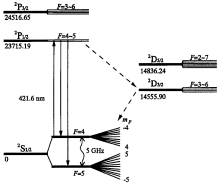
\includegraphics[width=8.6cm, keepaspectratio=true]{sff_1993-87Sr+.eps}
	\caption{Alkali-like energy levels of \Srion{87}{+}. Figure from \cite{sff_1993}.}
\end{figure}

The hyperfine splitting of the $\SLJ{2}{S}{1/2}$ was measured to be \SI{5002368.363(57)}{\kHz}, meaning the magnetic hyperfine constant was determined to be $A = \SI{-1000473.673(11)}{\kHz}$. 

\section{Electronic properties}

Strontium has two principal transitions from the $\nSLJ{5s^2}{1}{S}{0}$ ground state, one at \SI{461}{\nm} and another at \SI{689}{\nm}. 
The \SI{461}{\nm} transition is used for the blue MOT and absorption imaging while the \SI{689}{nm} transition is used for the red MOT and spectroscopy. 

\begin{table}[htbp]
	\centering
	\begin{tabular}{@{}ccccc@{}}
		\toprule
		Isotope						& Lower level									& Upper level					& $\Delta E_\text{iso}$	& Ref	\\
		\midrule
		\Sr{88}						& $\nSLJ{5s^2}{1}{S}{0}$						& $\nSLJ{5s5p}{1}{P}{1}$		&						&		\\
		\Sr{87}						& $\nSLJF{5s^2}{1}{S}{0}{9/2}$					& $\nSLJF{5s5p}{1}{P}{1}{7/2}$	&						&		\\
									&												& $\nSLJF{5s5p}{1}{P}{1}{11/2}$	&						&		\\
									&												& $\nSLJF{5s5p}{1}{P}{1}{9/2}$	&						&		\\
		\Sr{86}						& $\nSLJ{5s^2}{1}{S}{0}$						& $\nSLJ{5s5p}{1}{P}{1}$		&						&		\\
		\Sr{84}						& $\nSLJ{5s^2}{1}{S}{0}$						& $\nSLJ{5s5p}{1}{P}{1}$		&						&		\\
		\bottomrule
	\end{tabular}
	\caption{\label{tab:blue_isotope_shift}xxxxxxxx.}
\end{table}

*************************************************

\begin{table}[H]
\centering
\begin{tabular}{|l|l|l|l|l|}
\hline
Isotope 	& Lower level    				& Upper level 					& Frequency {[}kHz{]} 	& References 						\\ \hline
\Sr{88} 	& $\nSLJ{5s^2}{1}{S}{0}$ 		& $\nSLJ{5s5p}{1}{P}{1}$ 		&                     	& 						           	\\ \hline
\Sr{87} 	& $\nSLJF{5s^2}{1}{S}{0}{9/2}$ 	& $\nSLJF{5s5p}{1}{P}{1}{7/2}$ 	&                     	& 									\\
			& $\nSLJF{5s^2}{1}{S}{0}{9/2}$ 	& $\nSLJF{5s5p}{1}{P}{1}{9/2}$ 	&                     	& 									\\
			& $\nSLJF{5s^2}{1}{S}{0}{9/2}$ 	& $\nSLJF{5s5p}{1}{P}{1}{11/2}$ &                     	&									\\ \hline
\Sr{86} 	& $\nSLJ{5s^2}{1}{S}{0}$ 		& $\nSLJ{5s5p}{1}{P}{1}$ 		&                     	& 									\\ \hline
\Sr{84} 	& $\nSLJ{5s^2}{1}{S}{0}$ 		& $\nSLJ{5s5p}{1}{P}{1}$ 		&                     	&			 						\\ \hline
\end{tabular}
\caption{Isotopic transition frequencies of the 461 nm line.}
\label{blue_iso_freq}
\end{table}

\subsection{Strontium isotope shifts}

Strontium has two principal transitions from the $\nSLJ{5s^2}{1}{S}{0}$ ground state, one at \SI{461}{\nm} and another at \SI{689}{\nm}. 

\subsection{689 nm transition}

\begin{table}[H]
\centering
\begin{tabular}{|c|c|c|l|}
\hline
Isotope						& Lower level									& Upper level										& \multicolumn{1}{c|}{Frequency [\si{kHz}]}							\\ \hline
\multirow{5}{*}{\Sr{88}}	& \multirow{5}{*}{$\nSLJ{5s^2}{1}{S}{0}$}		& \multirow{5}{*}{$\nSLJ{5s5p}{3}{P}{1}$}			& \num{434829121311 +- 10} \cite{Sansonetti_2010, Ferrari_2003}		\\ %\cline{4-4}
							&												&													& \num{434829121300 +- 20} \cite{Courtillot_2005}					\\ %\cline{4-4}
							&												&													& \num{434829121312.334 +- 0.039} \cite{Ido_2005}					\\ %\cline{4-4}
							&												&													& \num{434829121313 +- 20} \cite{Hui_2015}							\\ \cline{4-4}
							&												&													& \num{434829121312.334 +- 0.039}									\\ \hline
\multirow{9}{*}{\Sr{87}}	& \multirow{3}{*}{$\nSLJF{5s^2}{1}{S}{0}{9/2}$}	& \multirow{3}{*}{$\nSLJF{5s5p}{3}{P}{1}{7/2}$}		& \num{434830473270 +- 55} \cite{Sansonetti_2010, Courtillot_2005}	\\ %\cline{4-4}
							&												&													& \num{434830473218 +- 55} \cite{Hui_2015}							\\ \cline{4-4}
							&												&													& \num{434830473244 +- 39}											\\ \cline{2-4}
							& \multirow{3}{*}{$\nSLJF{5s^2}{1}{S}{0}{9/2}$}	& \multirow{3}{*}{$\nSLJF{5s5p}{3}{P}{1}{9/2}$}		& \num{434829343010 +- 50} \cite{Sansonetti_2010, Courtillot_2005}	\\ %\cline{4-4}
							&												&													& \num{434829342986 +- 65} \cite{Hui_2015}							\\ \cline{4-4}
							&												&													& \num{434829343001 +- 40}											\\ \cline{2-4}
							& \multirow{3}{*}{$\nSLJF{5s^2}{1}{S}{0}{9/2}$}	& \multirow{3}{*}{$\nSLJF{5s5p}{3}{P}{1}{11/2}$}	& \num{434827879860 +-55} \cite{Sansonetti_2010, Courtillot_2005}	\\ %\cline{4-4}
							&												&													& \num{434827879826 +- 60} \cite{Hui_2015}							\\ \cline{4-4}
							&												&													& \num{434827879844 +- 41}											\\ \hline
\multirow{3}{*}{\Sr{86}}	& \multirow{3}{*}{$\nSLJ{5s^2}{1}{S}{0}$}		& \multirow{3}{*}{$\nSLJ{5s5p}{3}{P}{1}$}			& \num{434828957494 +- 10} \cite{Sansonetti_2010, Ferrari_2003}		\\ %\cline{4-4}
							&												&													& \num{434828957493 +- 25} \cite{Hui_2015}							\\ \cline{4-4}
							&												&													& \num{434828957493.9 +- 9.3}**										\\ \hline
\Sr{84}						& $\nSLJ{5s^2}{1}{S}{0}$						& $\nSLJ{5s5p}{3}{P}{1}$							& \num{434828769718 +- 111} \cite{Hui_2015}							\\ \hline
\end{tabular}
\caption{Absolute transition frequencies of the 689 nm intercombination line.}
\label{red_iso_freq}
\end{table}


\chapter{Optical Dipole Traps}

Put ODT details here.

\section{Optical Dipole Potential}

**** The derivation below loosely follows that found in \cite{Steck.QuantumAtomOptics, Ludlow2008.PhD} ****

For a two-level atom with ground (excited) state $\ket{g}$ ($\ket{e}$) with energy $E_{g} = \hbar \omega_{g}$ ($E_{e} = \hbar \omega_{e}$), the atomic Hamiltonian $H_{A}$ can be written as
\begin{equation}
	H_{A}	=	\hbar
				\begin{pmatrix}
					\omega_{e}	&	0			\\
					0			&	\omega_{g}
				\end{pmatrix}
\end{equation}
** Somehow introduce $\vb{d}\cdot\vb{E} \rightarrow \Omega \exp(-\iu \omega_{L} t)$ **
Introducing a laser at frequency $\omega$ which couples $\ket{g}$ and $\ket{e}$ and can be represented by
\begin{equation}
	H_{AF}	=	\frac{\hbar}{2}
				\begin{pmatrix}
					0							&	\Omega \cos(\omega t)	\\
					\Omega^{*} \cos(\omega t)	&	0
				\end{pmatrix}
\end{equation}
Using the unitary transformation
\begin{equation}
	U	=	\begin{pmatrix}
				\me^{\iu \omega t}	&	0	\\
				0					&	1
			\end{pmatrix}
\end{equation}
the total (transformed) Hamiltonian for the system can be written as
\begin{equation}
	\widetilde{H}	=		\hbar
							\begin{pmatrix}
								-\Delta												&	\frac{\Omega}{2} \qty(1 + \me^{\iu 2 \omega t})	\\
								\frac{\Omega^{*}}{2} \qty(1 + \me^{-\iu 2 \omega t})	&	\omega_{g}
							\end{pmatrix}
					\approx	\hbar
							\begin{pmatrix}
								-\Delta					&	\frac{\Omega}{2}	\\
								\frac{\Omega^{*}}{2}	&	\omega_{g}
							\end{pmatrix}
\end{equation}
where $\Delta \equiv \omega - \omega_{e}$ and the rotating wave approximation (RWA) was made ** clarify why/how the RWA is done **.

For $\Delta \gg \Omega$, ..... continue deriving...
\chapter{Tips and Tricks}
\label{ap:tips_n_tricks}

Various tips and tricks I picked up over the years. 

\section{Working with (high-power) fibers}

Notes about fibered ODT setup.

Having a fiber inspection scope is super helpful\footnote{We recently acquired a F1MS200U from Fiber Instrument Sales and FS201-PM from Thorlabs.}

\section{Fiber injection lock slave lasers}

We found that using a fiber to couple injection light to a slave laser greatly increased the flexibility and ease-of-use of the slave laser. Fibering the injection light greatly shortens the path lengths compared to free-space injection locking. The fiber also enables easier optimization of the injection lock by using the light back-coupled through the fiber (exiting the ``input'' end) to optimize alignment to the diode. 

\section{Scanning the UV laser}
\label{ap:scanning_uv_laser}

**Talk about how we used to flip-flop sidebands to patch together the $n=98-99$ scan but then the new synthesizer allows us to continue scanning once we hop over the transfer cavity crossing.**

Our current transfer cavity has an FSR of about **\SI{300}{\MHz}** which means the sidebands cross every **\SI{150}{\MHz}**.

\subsection{Switching sidebands to increase scan range}

**Talk about how we used to flip-flop sidebands to patch together the $n=98-99$ scan but then the new synthesizer allows us to continue scanning once we hop over the transfer cavity crossing.**

\subsection{``Continuous'' scanning of the transfer cavity}

**Using the new synthesizer, blah, blah, blah, we no longer have to switch EOM sidebands every FSR/2. 
If we want to scan a few GHz (limited by the synthesizer and RF amplifier ranges) we just need to hop over sideband crossings.**

%\include{append-a}
%\appendix
%\addcontentsline{toc} {chapter}{\numberline {}Appendix A}
%\include{append-a}
%\include{append-b}
%\addcontentsline{toc} {chapter}{\numberline {}Bibliography}{}
%\include{biblio}

%%%%%%%%%%%%%%%%%%%%%%%%%%%%%%%%%%%%%%%%%%%%%%%%%%
% Bibliography

%\bibliographystyle{ieeetr}
%\bibliography{bibliography}
\addcontentsline{toc}{chapter}{Bibliography}
\printbibliography

\end{document}
